\documentclass[11pt,a4paper]{article}
\usepackage[utf8]{inputenc}
\usepackage[T1]{fontenc}
\usepackage{amsmath,amssymb,amsfonts}
\usepackage{graphicx}
\usepackage{booktabs}
\usepackage{hyperref}
\usepackage{xcolor}
\usepackage{geometry}
\usepackage{fancyhdr}
\usepackage{titlesec}
\usepackage{enumitem}
\usepackage{float}
\usepackage{caption}
\usepackage{subcaption}
\usepackage{listings}
\usepackage{tikz}
\usetikzlibrary{shapes,arrows,positioning,fit,backgrounds,calc}

\geometry{margin=1in}

% Colors
\definecolor{qnkblue}{RGB}{30,90,150}
\definecolor{qnkgold}{RGB}{180,140,40}
\definecolor{codebg}{RGB}{245,245,245}
\definecolor{qnkgreen}{RGB}{40,140,60}
\definecolor{qnkred}{RGB}{180,40,40}

% Hyperref setup
\hypersetup{
    colorlinks=true,
    linkcolor=qnkblue,
    filecolor=qnkblue,
    urlcolor=qnkblue,
    citecolor=qnkblue
}

% Title formatting
\titleformat{\section}{\Large\bfseries\color{qnkblue}}{\thesection}{1em}{}
\titleformat{\subsection}{\large\bfseries\color{qnkblue!80}}{\thesubsection}{1em}{}
\titleformat{\subsubsection}{\normalsize\bfseries\color{qnkblue!60}}{\thesubsubsection}{1em}{}

% Header/Footer
\pagestyle{fancy}
\fancyhf{}
\fancyhead[L]{\small\color{gray}Q-NarwhalKnight Node Operator Guide}
\fancyhead[R]{\small\color{gray}v2.0}
\fancyfoot[C]{\thepage}
\renewcommand{\headrulewidth}{0.4pt}

% Code listing style
\lstset{
    backgroundcolor=\color{codebg},
    basicstyle=\ttfamily\small,
    breaklines=true,
    frame=single,
    rulecolor=\color{gray!30},
    keywordstyle=\color{qnkblue}\bfseries,
    stringstyle=\color{qnkgreen},
    commentstyle=\color{gray},
    numbers=left,
    numberstyle=\tiny\color{gray},
    numbersep=5pt
}

\begin{document}

% Title Page
\begin{titlepage}
\centering
\vspace*{2cm}

{\Huge\bfseries\color{qnkblue} Q-NarwhalKnight\\[0.5cm]}
{\LARGE\color{qnkblue!80} Node Operator Guide\\[0.2cm]}
{\Large\color{gray} Zero-Config Setup, Fee Structure,\\[0.2cm] Admin Wallet \& OAuth2 Wallet Linking\\[2cm]}

{\large\bfseries v2.0\\[0.5cm]}
{\large March 2026\\[3cm]}

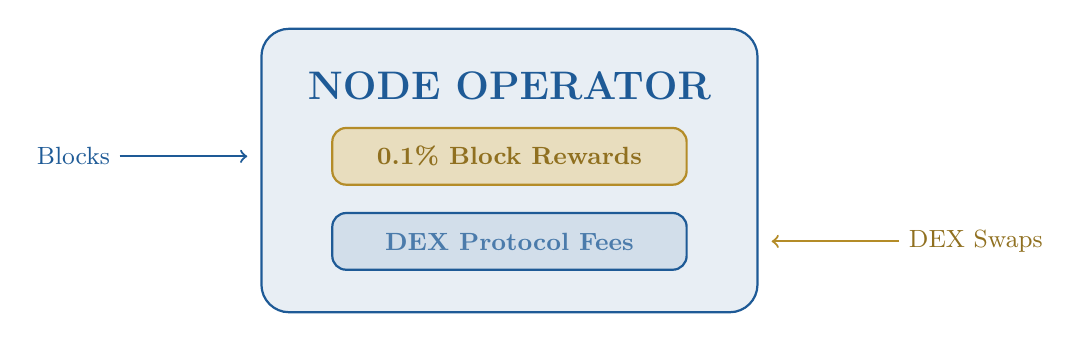
\begin{tikzpicture}[scale=0.9]
    % Node operator visualization
    \draw[fill=qnkblue!10, draw=qnkblue, thick, rounded corners=10pt] (-3.5,-2) rectangle (3.5,2);
    \node[font=\Large\bfseries, color=qnkblue] at (0,1.2) {NODE OPERATOR};
    \draw[fill=qnkgold!30, draw=qnkgold, thick, rounded corners=5pt] (-2.5,-0.2) rectangle (2.5,0.6);
    \node[font=\small\bfseries, color=qnkgold!80!black] at (0,0.2) {0.1\% Block Rewards};
    \draw[fill=qnkblue!20, draw=qnkblue, thick, rounded corners=5pt] (-2.5,-1.4) rectangle (2.5,-0.6);
    \node[font=\small\bfseries, color=qnkblue!80] at (0,-1.0) {DEX Protocol Fees};

    % Arrows from left (blocks)
    \draw[->, thick, color=qnkblue] (-5.5,0.2) -- (-3.7,0.2);
    \node[font=\small, color=qnkblue, left] at (-5.5,0.2) {Blocks};

    % Arrows from right (swaps)
    \draw[->, thick, color=qnkgold] (5.5,-1.0) -- (3.7,-1.0);
    \node[font=\small, color=qnkgold!80!black, right] at (5.5,-1.0) {DEX Swaps};
\end{tikzpicture}

\vfill

{\small\color{gray} Quillon Blockchain Project \textbullet\ \url{https://quillon.xyz}}

\end{titlepage}

% Abstract
\begin{abstract}
Q-NarwhalKnight (QNK) is a quantum-resistant blockchain with a DAG-Knight consensus engine.
Node operators who run public-facing QNK nodes earn \textbf{0.1\% of every block reward}
credited directly to their configured admin wallet, plus a share of DEX protocol fees.
As of v8.6.5, new operators can spin up a fully-configured node \emph{in under 60 seconds}
using the built-in \textbf{Setup Wizard}---no manual environment variables, no hand-written
systemd files.
This guide covers the zero-config setup wizard, hardware requirements, installation,
admin wallet configuration, the 2\% development fee structure, OAuth2 device-login
wallet linking for miners, the admin API, and the TUI monitoring dashboard.
\end{abstract}

\tableofcontents
\newpage

%----------------------------------------------------------------------
\section{Introduction}
%----------------------------------------------------------------------

The QNK network relies on a distributed set of bootstrap and relay nodes that
store the full blockchain, serve API requests to wallets and miners, relay
blocks via libp2p gossipsub, and facilitate turbo-sync for new peers.

Running a node is voluntary, but the protocol now \emph{rewards} operators
with a share of the development fee embedded in every coinbase transaction.
This creates a sustainable incentive for decentralised infrastructure
without requiring staking locks or delegation mechanics.

\subsection{Why Run a Node?}

\begin{itemize}[nosep]
    \item \textbf{Earn passive income} -- 0.1\% of every block reward is credited to your wallet.
    \item \textbf{Earn DEX fees} -- 0.05\% of every swap on the built-in DEX is shared with operators.
    \item \textbf{Strengthen the network} -- more nodes means faster sync, better geographic coverage, and higher censorship resistance.
    \item \textbf{First-class citizen} -- operators get the admin API, real-time TUI dashboard, and direct P2P connectivity.
\end{itemize}

%----------------------------------------------------------------------
\section{System Requirements}
%----------------------------------------------------------------------

\begin{table}[H]
\centering
\begin{tabular}{@{}lll@{}}
\toprule
\textbf{Resource} & \textbf{Minimum} & \textbf{Recommended} \\
\midrule
RAM        & 4\,GB              & 8\,GB+ \\
Disk       & 50\,GB SSD         & 100\,GB+ NVMe \\
CPU        & 2 cores x86\_64    & 4+ cores \\
Network    & 10\,Mbps stable    & 100\,Mbps \\
OS         & Linux x86\_64      & Ubuntu 22.04+ / Debian 12+ \\
\bottomrule
\end{tabular}
\caption{Hardware requirements for a QNK node.}
\end{table}

\subsection{Network Ports}

\begin{table}[H]
\centering
\begin{tabular}{@{}llp{7cm}@{}}
\toprule
\textbf{Port} & \textbf{Protocol} & \textbf{Purpose} \\
\midrule
8080 & TCP/HTTP  & REST API, SSE streaming, miner submissions, wallet queries \\
9001 & TCP/QUIC  & libp2p gossipsub P2P -- block relay, peer discovery (Kademlia DHT) \\
\bottomrule
\end{tabular}
\caption{Required network ports (open in firewall).}
\end{table}

%----------------------------------------------------------------------
\section{Installation \& First Boot}
%----------------------------------------------------------------------

\subsection{Download the Binary}

\begin{lstlisting}[language=bash,title={Download and start (one command)}]
# Download the latest release
wget https://quillon.xyz/downloads/q-api-server-linux-x86_64
chmod +x q-api-server-linux-x86_64

# Just run it -- the Setup Wizard handles the rest
./q-api-server-linux-x86_64 --port 8080
\end{lstlisting}

On first boot (no \texttt{.env} file detected), the \textbf{Setup Wizard} launches
automatically. It takes roughly 60 seconds and requires no terminal expertise.
See Section~\ref{sec:setup-wizard} for the full flow.

If you prefer manual configuration, pass \texttt{--admin-wallet}:

\begin{lstlisting}[language=bash,title={Manual start (skips wizard)}]
./q-api-server-linux-x86_64 --port 8080 \
    --admin-wallet <YOUR_64_CHAR_HEX_WALLET>
\end{lstlisting}

After setup completes, the node will:
\begin{enumerate}[nosep]
    \item Load configuration from the generated \texttt{.env} file.
    \item Create the data directory (\texttt{data-mainnet-genesis/} by default).
    \item Generate a unique libp2p identity key.
    \item Connect to bootstrap peers via Kademlia DHT.
    \item Begin syncing the blockchain (turbo-sync for fast catch-up).
\end{enumerate}

\subsection{Environment Variables}

The Setup Wizard writes these automatically, but you can override any value
by editing \texttt{.env} or setting shell environment variables.

\begin{table}[H]
\centering
\begin{tabular}{@{}llp{6cm}@{}}
\toprule
\textbf{Variable} & \textbf{Default} & \textbf{Description} \\
\midrule
\texttt{Q\_ADMIN\_WALLET} & founder wallet & 64-char hex address receiving operator fees \\
\texttt{Q\_NETWORK\_ID} & \texttt{mainnet-genesis} & Network identifier (prevents cross-chain contamination) \\
\texttt{Q\_DB\_PATH} & \texttt{./data-\{network\}} & Database storage directory \\
\texttt{Q\_NODE\_OPERATOR\_FEE\_PROMILLE} & \texttt{50} & Operator share in per-mille of dev fee (50 = 5\%) \\
\texttt{ROCKSDB\_BLOCK\_CACHE\_MB} & auto & RocksDB block cache size (auto-tuned by hardware tier) \\
\texttt{Q\_PREFLIGHT\_CHECK} & \texttt{1} & Run database integrity check on startup \\
\texttt{Q\_TURBO\_SYNC} & \texttt{1} & Enable batched P2P blockchain sync \\
\texttt{Q\_BOOTSTRAP\_URL} & \texttt{https://quillon.xyz} & Bootstrap server for setup wizard config fetch \\
\bottomrule
\end{tabular}
\caption{Key environment variables (auto-configured by Setup Wizard).}
\end{table}

%----------------------------------------------------------------------
\section{Setup Wizard (Zero-Config First Boot)}
\label{sec:setup-wizard}
%----------------------------------------------------------------------

Starting with v8.6.5, the QNK node ships with an integrated \textbf{Setup Wizard}
that eliminates manual configuration entirely. New operators download the binary,
run it, approve a browser login, and the node is ready.

\subsection{When Does It Run?}

The wizard triggers automatically when \emph{all three} conditions are met:
\begin{enumerate}[nosep]
    \item No \texttt{.env} file exists in the working directory.
    \item No \texttt{--admin-wallet} CLI flag was provided.
    \item No \texttt{Q\_ADMIN\_WALLET} environment variable is set.
\end{enumerate}

You can also invoke it manually at any time:
\begin{lstlisting}[language=bash]
./q-api-server --setup
\end{lstlisting}

\subsection{What It Does (4 Steps)}

\begin{figure}[H]
\centering
\begin{tikzpicture}[
    node distance=0.5cm and 1.2cm,
    step/.style={draw, thick, rounded corners=5pt, minimum width=3.2cm,
                 minimum height=1.2cm, align=center, font=\small\bfseries},
    arr/.style={->, very thick, >=stealth, color=qnkblue}
]
    \node[step, fill=qnkblue!10, draw=qnkblue] (hw)
        {1. Detect\\Hardware};
    \node[step, fill=qnkblue!15, draw=qnkblue, right=of hw] (fetch)
        {2. Fetch\\Config};
    \node[step, fill=qnkgold!15, draw=qnkgold, right=of fetch] (login)
        {3. Browser\\Login};
    \node[step, fill=qnkgreen!15, draw=qnkgreen, right=of login] (write)
        {4. Write\\Config};

    \draw[arr] (hw) -- (fetch);
    \draw[arr] (fetch) -- (login);
    \draw[arr] (login) -- (write);
\end{tikzpicture}
\caption{Setup Wizard pipeline.}
\end{figure}

\begin{enumerate}
    \item \textbf{Detect Hardware} --- Reads RAM, CPU cores, and disk type
          (SSD vs HDD via \texttt{/sys/block/*/queue/rotational}).
          Maps to a hardware tier:

    \begin{table}[H]
    \centering
    \begin{tabular}{@{}llr@{}}
    \toprule
    \textbf{Tier} & \textbf{RAM Range} & \textbf{Cache (MB)} \\
    \midrule
    Low    & $\leq$ 4\,GB    & 512 \\
    Medium & 4--8\,GB        & 1024 \\
    High   & 8--32\,GB       & 2048 \\
    XLarge & $>$ 32\,GB      & 4096 \\
    \bottomrule
    \end{tabular}
    \caption{Hardware tier mapping.}
    \end{table}

    If an HDD is detected, \texttt{Q\_CHEAP\_SSD=1} is automatically enabled
    to reduce write amplification.

    \item \textbf{Fetch Bootstrap Config} --- Contacts the bootstrap server at\\
          \texttt{GET https://quillon.xyz/api/v1/node-config} to retrieve
          the current network ID, bootstrap peer addresses, and recommended
          environment variables. If the bootstrap is unreachable, sensible
          defaults are used.

    \item \textbf{Browser Login (OAuth2 Device Flow)} --- Opens a browser tab at\\
          \texttt{https://quillon.xyz/miner-login?code=XXXX} where you log in
          with your wallet. The wizard polls the server every 3 seconds (up to
          10 minutes) until your wallet address is confirmed. If login is
          skipped, the node starts with the founder wallet and you can set
          \texttt{Q\_ADMIN\_WALLET} in \texttt{.env} later.

    \item \textbf{Write Configuration} --- Generates two files:
    \begin{itemize}[nosep]
        \item \texttt{.env} --- all environment variables, hardware-tuned.
        \item \texttt{q-api-server.service} --- a systemd unit file.
              If running as root, it is installed to
              \texttt{/etc/systemd/system/} and auto-enabled.
              If not root, it is saved locally with manual install instructions.
    \end{itemize}
\end{enumerate}

\subsection{Re-running Setup}

The wizard is \textbf{idempotent}. Re-running \texttt{--setup} backs up
the existing \texttt{.env} to \texttt{.env.backup} before overwriting.
Your data directory and blockchain state are never touched.

\subsection{Example .env Output}

\begin{lstlisting}[title={Auto-generated .env}]
# Q-NarwhalKnight Node Configuration
# Auto-generated by setup wizard on 2026-03-01 14:30:00 UTC

# Network
Q_NETWORK_ID=mainnet-genesis
Q_DB_PATH=./data-mainnet-genesis

# Node admin wallet (controls admin panel)
Q_ADMIN_WALLET=qnka1b2c3d4e5f6...

# Safety & Sync
Q_PREFLIGHT_CHECK=1
Q_TURBO_SYNC=1
Q_BATCHED_WRITES=1
Q_STATE_SYNC=1
Q_IS_VALIDATOR=true
Q_P2P_PORT=9001

# Hardware-tuned (auto-detected)
ROCKSDB_BLOCK_CACHE_MB=2048

# Recommended by bootstrap server
Q_GOSSIPSUB_HEARTBEAT_MS=300
Q_TURBO_CHUNK_SIZE=500
\end{lstlisting}

\subsection{Systemd Service}

The generated service file uses \texttt{EnvironmentFile=} to load \texttt{.env},
making it easy to tune settings without editing the unit file:

\begin{lstlisting}[language=bash,title={Managing the service}]
# Start the node
sudo systemctl start q-api-server

# View logs
journalctl -u q-api-server -f

# Edit configuration (then restart)
nano .env
sudo systemctl restart q-api-server
\end{lstlisting}

%----------------------------------------------------------------------
\section{Admin Wallet Configuration}
%----------------------------------------------------------------------

The \textbf{admin wallet} is the operator's on-chain identity. All operator
fee rewards are credited to this address. It is set once at startup and
persists in-memory for the lifetime of the process.

\subsection{Setting the Admin Wallet}

There are two methods, listed in priority order:

\begin{enumerate}
    \item \textbf{CLI flag} (highest priority):\\
        \texttt{./q-api-server --admin-wallet abcd1234...}
    \item \textbf{Environment variable}:\\
        \texttt{Q\_ADMIN\_WALLET=abcd1234...}
\end{enumerate}

If neither is provided, the node defaults to the \emph{founder wallet},
meaning all dev fee revenue goes to the project founder. To earn operator
rewards, you \textbf{must} set your own wallet address.

\subsection{Address Format}

\begin{itemize}[nosep]
    \item 64 hexadecimal characters (32 bytes), case-insensitive.
    \item Optional \texttt{qnk} or \texttt{qug} prefix is automatically stripped.
    \item Example: \texttt{a1b2c3d4e5f6...} (64 chars total).
\end{itemize}

\subsection{Verification}

After starting the node, verify your admin wallet is active:

\begin{lstlisting}[language=bash,title={Check admin status}]
curl -s http://localhost:8080/api/v1/admin/is-admin
# Returns: {"is_admin": true, "wallet": "a1b2c3d4..."}
\end{lstlisting}

%----------------------------------------------------------------------
\section{Fee Structure \& Economics}
%----------------------------------------------------------------------

Every block produced by the network includes \textbf{coinbase transactions}
that distribute the block reward. The fee split is enforced at the consensus
level --- blocks without correct fee transactions are rejected.

\subsection{Fee Flow Diagram}

\begin{figure}[H]
\centering
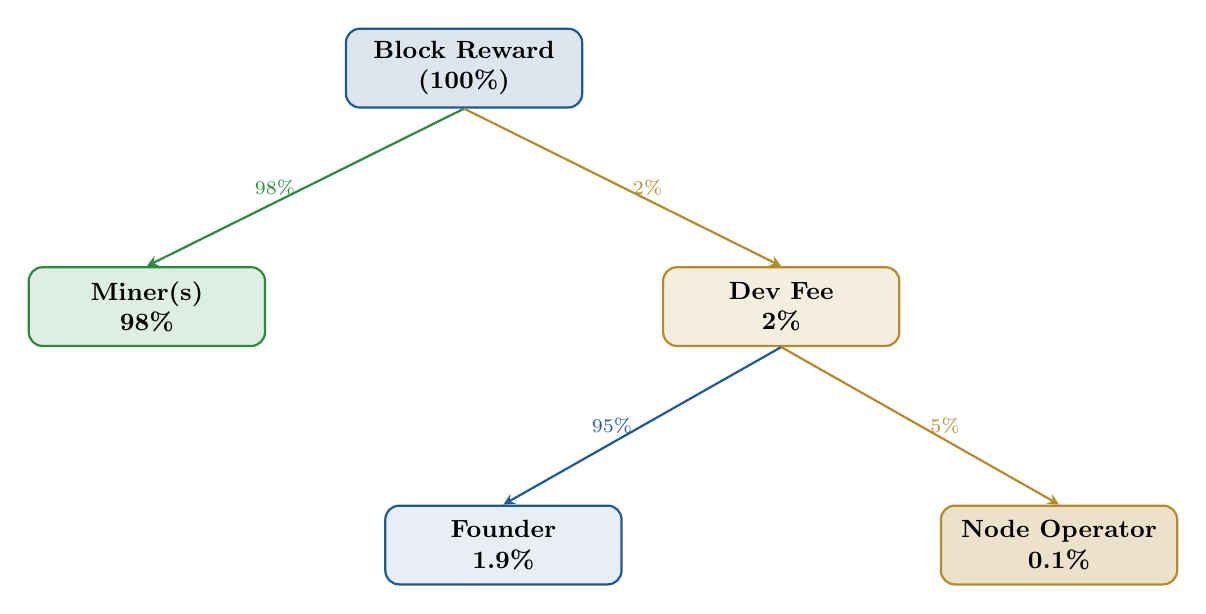
\begin{tikzpicture}[
    node distance=1.5cm,
    box/.style={draw, thick, rounded corners=5pt, minimum width=3cm,
                minimum height=1cm, align=center, font=\small\bfseries},
    arr/.style={->, thick, >=stealth}
]
    % Block Reward
    \node[box, fill=qnkblue!15, draw=qnkblue] (reward) {Block Reward\\(100\%)};

    % Miner
    \node[box, fill=qnkgreen!15, draw=qnkgreen, below left=2cm and 1cm of reward] (miner)
        {Miner(s)\\98\%};

    % Dev Fee
    \node[box, fill=qnkgold!15, draw=qnkgold, below right=2cm and 1cm of reward] (devfee)
        {Dev Fee\\2\%};

    % Founder
    \node[box, fill=qnkblue!10, draw=qnkblue, below left=2cm and 0.5cm of devfee] (founder)
        {Founder\\1.9\%};

    % Operator
    \node[box, fill=qnkgold!25, draw=qnkgold, below right=2cm and 0.5cm of devfee] (operator)
        {Node Operator\\0.1\%};

    % Arrows
    \draw[arr, color=qnkgreen] (reward.south) -- (miner.north)
        node[midway, left, font=\scriptsize] {98\%};
    \draw[arr, color=qnkgold] (reward.south) -- (devfee.north)
        node[midway, right, font=\scriptsize] {2\%};
    \draw[arr, color=qnkblue] (devfee.south) -- (founder.north)
        node[midway, left, font=\scriptsize] {95\%};
    \draw[arr, color=qnkgold] (devfee.south) -- (operator.north)
        node[midway, right, font=\scriptsize] {5\%};
\end{tikzpicture}
\caption{Block reward distribution flow.}
\end{figure}

\subsection{Fee Breakdown}

\begin{table}[H]
\centering
\begin{tabular}{@{}lrrr@{}}
\toprule
\textbf{Recipient} & \textbf{\% of Reward} & \textbf{BPS} & \textbf{Example (1.0 QUG block)} \\
\midrule
Miner(s)       & 98.0\%  & 9800  & 0.980000 QUG \\
Founder        & 1.9\%   & 190   & 0.019000 QUG \\
Node Operator  & 0.1\%   & 10    & 0.001000 QUG \\
\midrule
\textbf{Total} & 100.0\% & 10000 & 1.000000 QUG \\
\bottomrule
\end{tabular}
\caption{Fee breakdown with example amounts.}
\end{table}

\subsection{How Coinbase Transactions Encode the Split}

Each block contains up to three coinbase transactions:

\begin{enumerate}[nosep]
    \item \textbf{Founder fee TX} -- \texttt{from=0x00..00}, \texttt{to=founder\_wallet},
          amount = reward $\times$ 200/10000 $\times$ 950/1000 = 1.9\% of reward.
    \item \textbf{Operator fee TX} (if admin wallet configured) --
          \texttt{from=0x00..00}, \texttt{to=admin\_wallet},
          amount = reward $\times$ 200/10000 $\times$ 50/1000 = 0.1\% of reward.
    \item \textbf{Miner reward TX(s)} -- one per mining solution,
          amount = (reward $-$ dev\_fee) / num\_solutions.
\end{enumerate}

If no admin wallet is configured, the entire 2\% goes to the founder wallet.

\subsection{DEX Protocol Fee}

In addition to block rewards, node operators earn from the built-in
decentralised exchange:

\begin{itemize}[nosep]
    \item \textbf{0.05\%} (5 basis points) of every swap is collected as a protocol fee.
    \item This fee is separate from the AMM liquidity-provider fee.
    \item Revenue accrues to the node that processes the swap.
\end{itemize}

\subsection{Tracking Earnings}

Query your cumulative operator earnings via the admin API:

\begin{lstlisting}[language=bash,title={Check operator fee earnings}]
curl -s http://localhost:8080/api/v1/admin/fee-earnings
# {
#   "session_earnings_qug": "0.042000",
#   "total_earnings_qug": "1.250000",
#   "fee_tx_count": 1250,
#   "fee_rate_promille": 50
# }
\end{lstlisting}

%----------------------------------------------------------------------
\section{OAuth2 Device Login --- Web Wallet Linking}
%----------------------------------------------------------------------

Miners connect to your node and submit proof-of-work solutions. Before
mining begins, the miner must link its identity to a \texttt{quillon.xyz}
web wallet via the \textbf{OAuth2 Device Authorization Grant} flow
(RFC~8628).

\subsection{Purpose}

\begin{itemize}[nosep]
    \item Links the miner's hardware to a verified wallet address.
    \item Mining rewards are sent to the linked wallet.
    \item No private keys are exchanged --- only the public wallet address.
\end{itemize}

\subsection{Flow Diagram}

\begin{figure}[H]
\centering
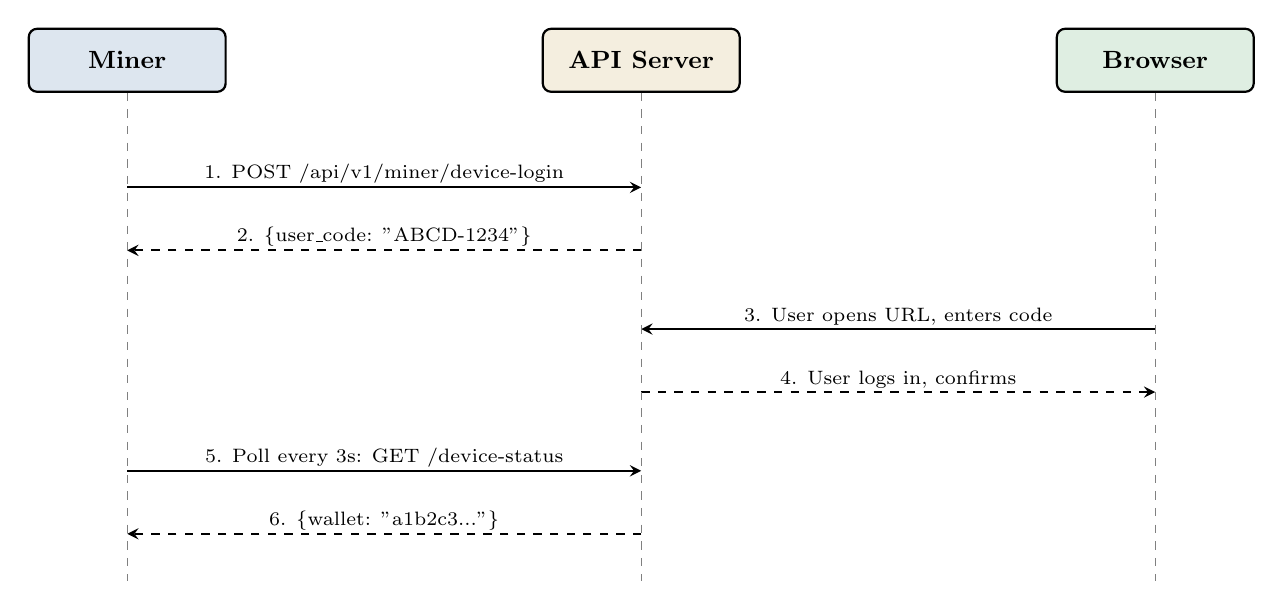
\begin{tikzpicture}[
    node distance=0.6cm,
    actor/.style={draw, thick, rounded corners=3pt, minimum width=2.5cm,
                  minimum height=0.8cm, align=center, font=\small\bfseries},
    msg/.style={->, thick, >=stealth},
    lbl/.style={font=\scriptsize, fill=white, inner sep=1pt}
]
    \node[actor, fill=qnkblue!15] (miner) {Miner};
    \node[actor, fill=qnkgold!15, right=4cm of miner] (api) {API Server};
    \node[actor, fill=qnkgreen!15, right=4cm of api] (browser) {Browser};

    % Step 1
    \draw[msg] ([yshift=-1.2cm]miner.south) -- ([yshift=-1.2cm]api.south)
        node[lbl, midway, above] {1. POST /api/v1/miner/device-login};

    % Step 2
    \draw[msg, dashed] ([yshift=-2.0cm]api.south) -- ([yshift=-2.0cm]miner.south)
        node[lbl, midway, above] {2. \{user\_code: "ABCD-1234"\}};

    % Step 3
    \draw[msg] ([yshift=-3.0cm]browser.south) -- ([yshift=-3.0cm]api.south)
        node[lbl, midway, above] {3. User opens URL, enters code};

    % Step 4
    \draw[msg, dashed] ([yshift=-3.8cm]api.south) -- ([yshift=-3.8cm]browser.south)
        node[lbl, midway, above] {4. User logs in, confirms};

    % Step 5 (poll)
    \draw[msg] ([yshift=-4.8cm]miner.south) -- ([yshift=-4.8cm]api.south)
        node[lbl, midway, above] {5. Poll every 3s: GET /device-status};

    % Step 6
    \draw[msg, dashed] ([yshift=-5.6cm]api.south) -- ([yshift=-5.6cm]miner.south)
        node[lbl, midway, above] {6. \{wallet: "a1b2c3..."\}};

    % Vertical lifelines
    \draw[gray, dashed] (miner.south) -- ([yshift=-6.2cm]miner.south);
    \draw[gray, dashed] (api.south) -- ([yshift=-6.2cm]api.south);
    \draw[gray, dashed] (browser.south) -- ([yshift=-6.2cm]browser.south);
\end{tikzpicture}
\caption{OAuth2 Device Authorization flow for miner wallet linking.}
\end{figure}

\subsection{Step-by-Step}

\begin{enumerate}
    \item \textbf{Miner requests a device code:}
\begin{lstlisting}[language=bash]
POST /api/v1/miner/device-login
# Response:
{
  "user_code": "ABCD-1234",
  "verification_url": "https://quillon.xyz/device",
  "expires_in": 600
}
\end{lstlisting}

    \item \textbf{Miner displays the code} to the user (TUI or GUI).

    \item \textbf{User opens the URL} in a browser and enters the code.

    \item \textbf{User logs in} to their quillon.xyz account (creates one if needed).

    \item \textbf{Miner polls} every 3 seconds:
\begin{lstlisting}[language=bash]
GET /api/v1/miner/device-status?code=ABCD-1234
# Pending:  {"status": "pending"}
# Complete: {"status": "complete", "wallet": "a1b2c3d4..."}
\end{lstlisting}

    \item \textbf{Mining begins} to the linked wallet address.
\end{enumerate}

\subsection{Security}

\begin{itemize}[nosep]
    \item Device codes expire after \textbf{10 minutes}.
    \item Wallet address format is validated (64 hex characters).
    \item The flow never exposes private keys --- only the public address is transmitted.
    \item Rate-limited to prevent brute-force code guessing.
\end{itemize}

%----------------------------------------------------------------------
\section{Admin API Reference}
%----------------------------------------------------------------------

All admin endpoints are accessible on \texttt{http://localhost:8080}. Some
require the request to originate from the admin wallet's authenticated session.

\begin{table}[H]
\centering
\small
\begin{tabular}{@{}llp{5.5cm}@{}}
\toprule
\textbf{Method} & \textbf{Endpoint} & \textbf{Description} \\
\midrule
GET  & \texttt{/api/v1/admin/is-admin}       & Check if current session is admin \\
GET  & \texttt{/api/v1/admin/settings}        & Retrieve node configuration \\
GET  & \texttt{/api/v1/admin/fee-earnings}    & Operator fee earnings (session + total) \\
GET  & \texttt{/api/v1/admin/operator-fees}   & Detailed fee history \\
GET  & \texttt{/api/v1/admin/dev-fee}         & Current dev fee rate (BPS) \\
GET  & \texttt{/api/v1/node/info}             & Node version, height, peers, uptime \\
GET  & \texttt{/api/v1/node/update-check}     & Check for binary updates \\
POST & \texttt{/api/v1/admin/settings}        & Update node settings (admin only) \\
\bottomrule
\end{tabular}
\caption{Admin API endpoints.}
\end{table}

%----------------------------------------------------------------------
\section{Node TUI Dashboard}
%----------------------------------------------------------------------

The QNK node includes a terminal user interface (TUI) for real-time monitoring.
Launch with \texttt{--tui} or press keys while the node is running in the foreground.

\subsection{Key Bindings}

\begin{table}[H]
\centering
\begin{tabular}{@{}cl@{}}
\toprule
\textbf{Key} & \textbf{Action} \\
\midrule
\texttt{D} & Dashboard (default view) \\
\texttt{L} & Live log viewer \\
\texttt{N} & Network peers and P2P status \\
\texttt{S} & Statistics (hashrate, blocks, rewards) \\
\texttt{F} & Physics simulation dashboard \\
\texttt{B} & Bounty program panel \\
\texttt{M} & Menu / settings \\
\texttt{T} & Toggle network throttle mode \\
\texttt{Q} & Quit gracefully \\
\bottomrule
\end{tabular}
\caption{TUI key bindings.}
\end{table}

\subsection{Operator Earnings Display}

When an admin wallet is configured, the TUI header bar shows:

\begin{lstlisting}[title={TUI header example}]
 QNK Node v8.6.2 | Height: 58,432 | Peers: 12
 Operator: a1b2...c3d4 | Earned: 0.042 QUG (session) | 1.25 QUG (total)
\end{lstlisting}

The blockchain panel also displays per-block operator fee credits as they occur.

%----------------------------------------------------------------------
\section{Monitoring \& Troubleshooting}
%----------------------------------------------------------------------

\subsection{Checking Fee Credits}

\begin{lstlisting}[language=bash,title={journalctl commands}]
# Check operator fee credits
journalctl -u q-api-server --since "1 hour ago" \
    | grep -E "Operator fee|OPERATOR_FEE"

# Check block production
journalctl -u q-api-server --since "5 min ago" \
    | grep -E "Block.*produced|NEW BLOCK"

# Check P2P connectivity
journalctl -u q-api-server --since "5 min ago" \
    | grep -E "peer.*connected|Gossipsub"
\end{lstlisting}

\subsection{Common Issues}

\begin{table}[H]
\centering
\small
\begin{tabular}{@{}lp{8cm}@{}}
\toprule
\textbf{Symptom} & \textbf{Solution} \\
\midrule
No peers connecting &
    Ensure port 9001 is open (TCP + UDP). Check firewall and NAT.
    Verify \texttt{Q\_NETWORK\_ID} matches the network. \\
Sync stuck &
    Check disk space. Restart with \texttt{ROCKSDB\_BLOCK\_CACHE\_MB=512} if
    low on RAM. Verify bootstrap peer is reachable. \\
Missing operator rewards &
    Confirm \texttt{--admin-wallet} is set and differs from founder wallet.
    Check \texttt{/api/v1/admin/is-admin}. \\
OOM killed &
    Add swap: \texttt{fallocate -l 4G /swapfile \&\& mkswap /swapfile \&\& swapon /swapfile}.
    Set \texttt{ROCKSDB\_BLOCK\_CACHE\_MB} to 512--2048. \\
\bottomrule
\end{tabular}
\caption{Common issues and solutions.}
\end{table}

\subsection{HA Deployment (Multi-Node Operators)}

Operators running multiple nodes can use the included HA deployment script
for zero-downtime rolling upgrades:

\begin{lstlisting}[language=bash,title={Rolling upgrade}]
# Build new binary
cargo build --release --package q-api-server

# Rolling deploy across all nodes
./scripts/ha-deploy.sh full -y

# Check status of all nodes
./scripts/ha-deploy.sh status
\end{lstlisting}

%----------------------------------------------------------------------
\section{Security}
%----------------------------------------------------------------------

\subsection{Signing Key Locality}

The node's libp2p identity key and any signing keys are generated locally
and \textbf{never leave the machine}. There is no key upload, no cloud HSM
dependency, and no custodial risk. Your node's identity is sovereign.

\subsection{Founder Wallet Protections}

The founder wallet (\texttt{efca...0723}) has additional consensus-enforced
safeguards:

\begin{itemize}[nosep]
    \item \textbf{Timelock}: Large withdrawals require a multi-block confirmation delay.
    \item \textbf{Vesting schedule}: Founder allocation unlocks gradually over 4 years.
    \item \textbf{Max withdrawal cap}: Single-transaction withdrawal limits prevent rug-pulls.
\end{itemize}

\subsection{Network Isolation}

Each network instance (\texttt{mainnet2026.1.1}, \texttt{testnet}, etc.) is
isolated by three mechanisms:

\begin{enumerate}[nosep]
    \item \textbf{Gossipsub topic namespacing}: \texttt{/qnk/\{network\_id\}/blocks}
    \item \textbf{Protocol handshake validation}: Peers reject mismatched \texttt{network\_id}
    \item \textbf{HTTP state sync}: \texttt{FullStateSnapshot} includes \texttt{network\_id} field
\end{enumerate}

This prevents cross-chain contamination even if nodes from different networks
share the same physical machine.

%----------------------------------------------------------------------
\section*{References}
%----------------------------------------------------------------------

\begin{enumerate}[nosep]
    \item Q-NarwhalKnight Privacy Layer Whitepaper v3.0, February 2026.\\
          \url{https://quillon.xyz/downloads/qnk-privacy-layer-whitepaper.pdf}
    \item Quillon Bank Aegis-QL Whitepaper, February 2026.\\
          \url{https://quillon.xyz/downloads/quillon_bank_aegis_ql_whitepaper.pdf}
    \item Apollo Sync Optimization Whitepaper, January 2026.\\
          \url{https://quillon.xyz/downloads/apollo-sync-optimization-whitepaper.pdf}
    \item RFC 8628 --- OAuth 2.0 Device Authorization Grant.\\
          \url{https://datatracker.ietf.org/doc/html/rfc8628}
    \item QNK K-Parameter Whitepaper.\\
          \url{https://quillon.xyz/downloads/K-Parameter_Whitepaper.pdf}
\end{enumerate}

\vspace{1cm}
\begin{center}
\color{gray}\rule{0.5\textwidth}{0.4pt}\\[0.5cm]
{\small\color{gray} \textcopyright\ 2026 Quillon Blockchain Project. All rights reserved.\\
For support, visit \url{https://quillon.xyz} or join our Discord community.}
\end{center}

\end{document}
